\section{Model interpretation}\label{sec:7}

\begin{disposition}
We interpret the final LightGBM model in four ways, going from the whole model down to a single week. For this section we train the final configuration on fold B's training years and explain its predictions for 2021, the validation year whose price level (75 EUR/MWh) is closest to the test years.
\end{disposition}

% Final text:


\subsection{Feature importance}\label{sec:7.1}

\begin{disposition}
Total gain per feature and per feature family. What to say: the relaxed-LP features account for about 80\% of the total gain, and ``LP: unit on'' alone for about half. Next come the unit ID, reservoir inflow, the DP regret and the calendar. Everything we built before the LP still contributes, but much less. This confirms the story of Section~\ref{sec:4}: the model's knowledge comes mainly from the optimisation. Caveat we will mention: gain importance does not show \emph{direction}, and it favours features that are used for the first, big splits.
\end{disposition}

% Final text:


\begin{figure}[H]
  \centering
  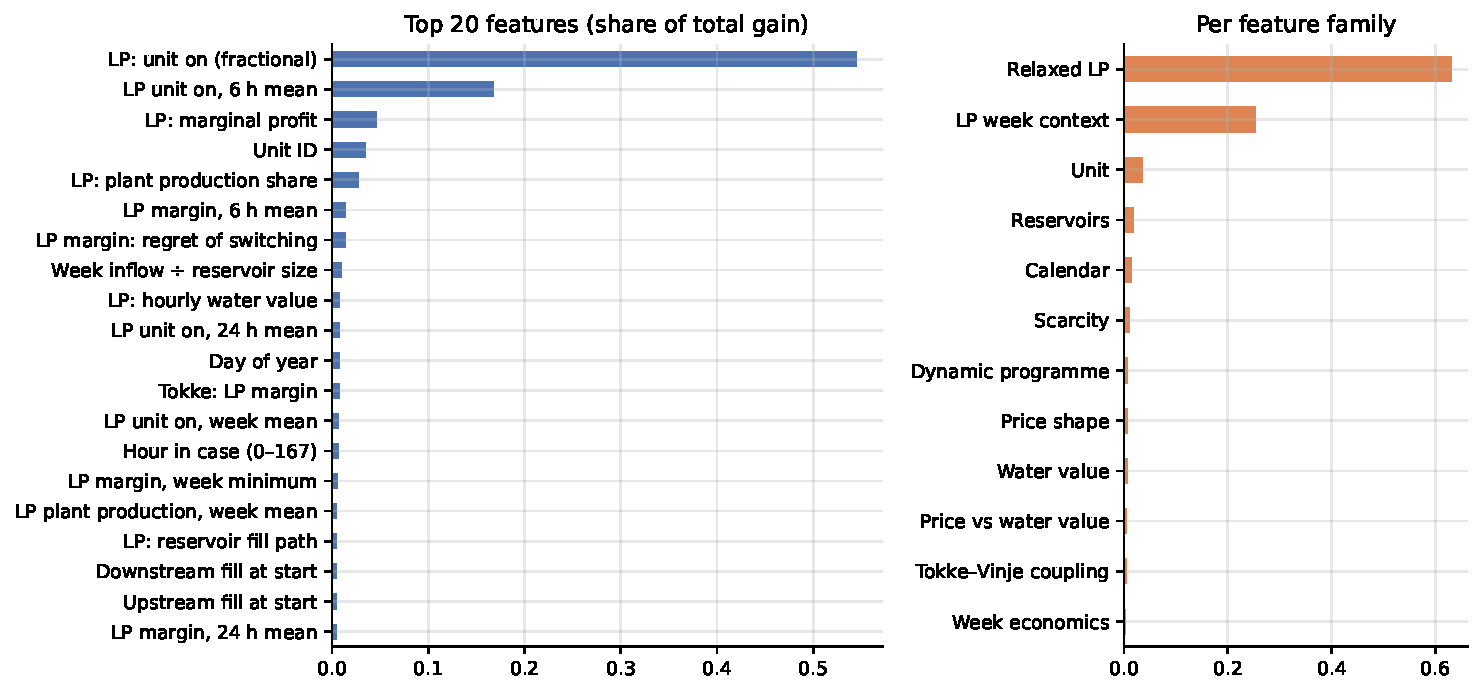
\includegraphics[width=\linewidth]{figures/fig_7_1.pdf}
  \caption{Gain importance, final LightGBM model (fold B)}
  \label{fig:7.1}
\end{figure}

\subsection{SHAP values}\label{sec:7.2}

\begin{disposition}
We will explain SHAP in plain words: for one prediction, SHAP splits the model's output (in log-odds) into a contribution from each feature, so that the contributions add up to the prediction. Averaging the absolute contributions gives an importance per feature, and plotting them against the feature value shows \emph{how} a feature pushes the prediction. Observations to describe:

\begin{itemize}
\tightlist
\item
  \emph{The two importance measures disagree on the top feature.} By gain, ``LP: unit on'' is first; by SHAP, ``LP: marginal profit'' is first (Figure~\ref{fig:7.2}). Explanation: gain measures how much the splits on a feature improve the training loss, and ``LP: unit on'' makes the first and biggest splits (clearly on vs clearly off). SHAP measures how much a feature moves \emph{each individual} prediction, and the marginal profit adjusts almost every prediction continuously, also inside the ``clearly on'' and ``clearly off'' groups.
\item
  \textbf{How to read Figure~\ref{fig:7.2}} (the report must explain this, because it is not intuitive). Each \emph{row} is one feature. Each \emph{dot} is one unit-hour (one unit in one hour of one case), and every unit-hour appears once in every row.

  \begin{itemize}
  \tightlist
  \item
    \emph{Position (left/right)} = what the feature did to the prediction for that unit-hour. Right of the zero line means the feature pushed that unit-hour towards ON (higher probability of running), left means it pushed it towards OFF. Far from zero = a strong push.
  \item
    \emph{Colour} = the feature's own value in that unit-hour, compared with its other values: blue = one of the lowest values of this feature, red = one of the highest. \textbf{Colour says nothing about whether the feature is good or bad, and nothing about the prediction by itself.}
  \item
    The meaning comes from combining the two. In the ``LP: marginal profit'' row, red dots are on the right: when the LP finds running very profitable, the model predicts ON. In the ``LP: hourly water value'' row it is the opposite: red dots are on the left, because when the water is very valuable the model predicts OFF (the water is saved).
  \item
    Why the rows look roughly mirrored: SHAP values are measured from the model's average prediction, so a useful feature pushes some unit-hours up and others down. Units are ON about half the time, so the two sides are about equally large. A wide two-sided row means the feature separates ON from OFF strongly, not that it cancels out.
  \item
    ``Unit ID'' is drawn in grey: the units are categories, so ``low'' and ``high'' values have no meaning.
  \end{itemize}
\end{itemize}
\end{disposition}

% Final text:


\begin{figure}[H]
  \centering
  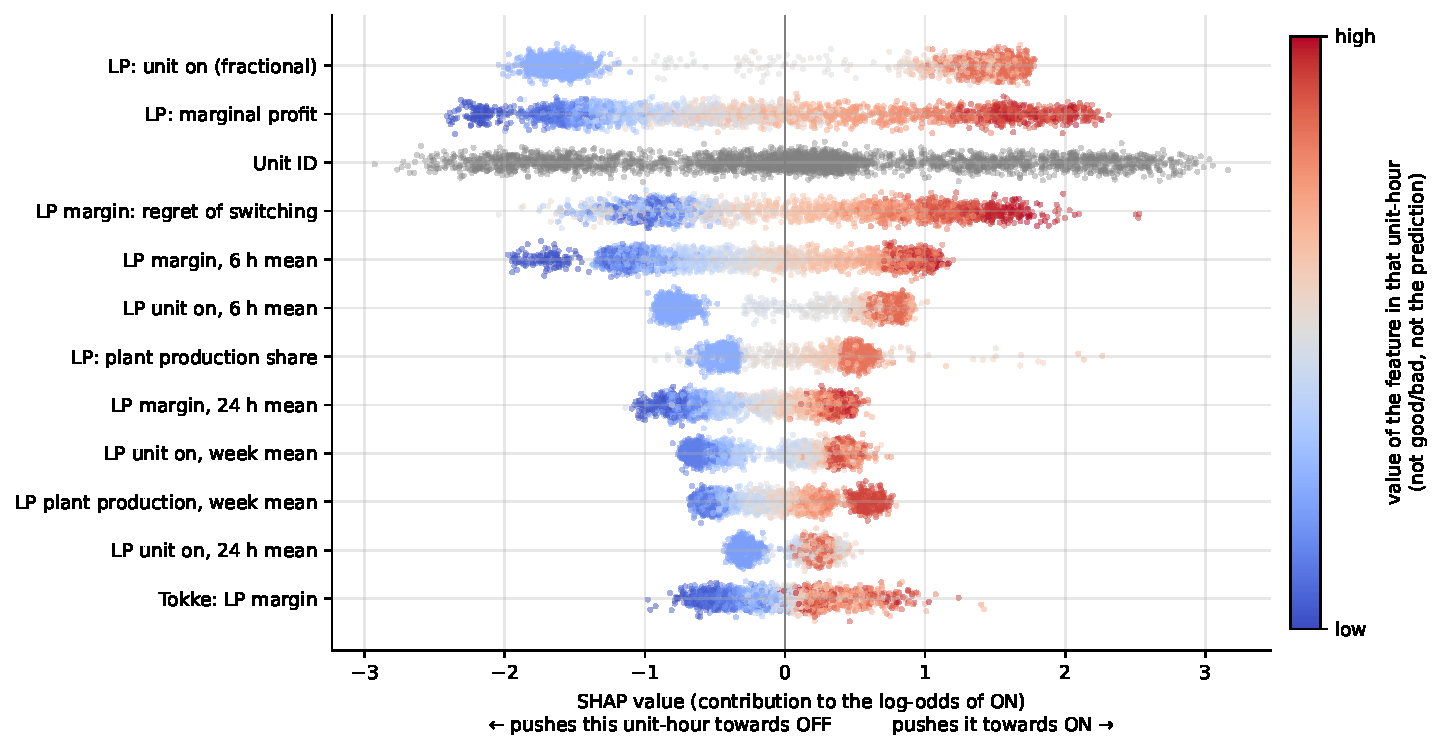
\includegraphics[width=\linewidth]{figures/fig_7_2.pdf}
  \caption{SHAP summary, top 12 features. Each dot is one unit-hour}
  \label{fig:7.2}
\end{figure}

\begin{disposition}
\begin{itemize}
\tightlist
\item
  \emph{The directions are physically sensible} (Figure~\ref{fig:7.2}). A high LP marginal profit, a high LP unit-on and a high LP production all push towards ON. A high LP water value pushes towards OFF (expensive water is saved). A high DP regret pushes towards ON.
\item
  \emph{The model trusts the LP but not blindly} (Figure~\ref{fig:7.3}). The effect of the LP's marginal profit is a smooth S-curve centred at zero: the model is most sensitive exactly where running is barely profitable or barely unprofitable. ``LP: unit on'' has clusters at 0 and 1 with fractional values in between that the model maps to intermediate probabilities.
\end{itemize}
\end{disposition}

% Final text:


\begin{figure}[H]
  \centering
  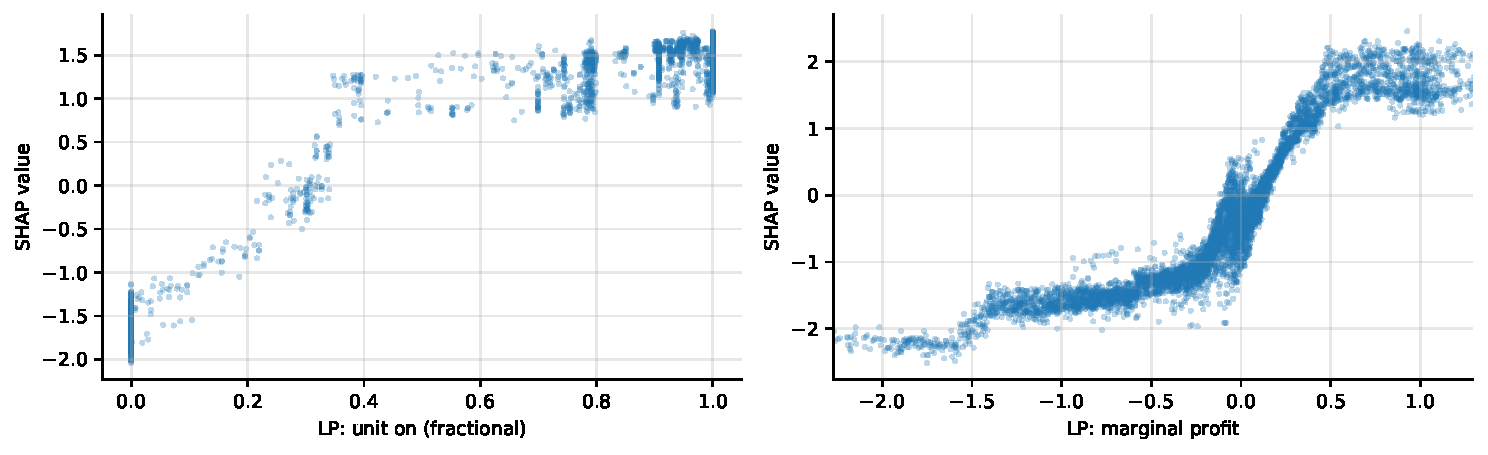
\includegraphics[width=\linewidth]{figures/fig_7_3.pdf}
  \caption{How the LP features push the prediction (fold B, 2021)}
  \label{fig:7.3}
\end{figure}

\begin{disposition}
\begin{itemize}
\tightlist
\item
  Note: we computed SHAP with LightGBM's built-in TreeSHAP (\texttt{pred\_contrib=True}) instead of the \texttt{shap} package.
\end{itemize}
\end{disposition}

% Final text:


\subsection{Where the model is right and wrong}\label{sec:7.3}

\begin{disposition}
\begin{itemize}
\tightlist
\item
  \emph{Per unit (Figure~\ref{fig:7.4}).} Most units score above 0.99. The hardest, with our explanations: Vinje G3 (0.950 in 2020; the third identical unit, so whether it runs is often a near-tie with G2, and it is on only 26\% of the time); Haukeli (0.97--0.98; a tiny 4.9 MW unit whose reservoir volume in the data is a constant placeholder, so neither we nor the LP know its real start state); Hogga (0.975--0.985; at the bottom of the cascade, so it depends on everything upstream); Lio in 2022 (0.972; driven by a minimum-flow requirement). 2020 is the hardest year for most units. Possible explanation: with prices near 9 EUR/MWh and water values near zero, many hours are close to indifferent, so small differences decide.
\end{itemize}
\end{disposition}

% Final text:


\begin{figure}[H]
  \centering
  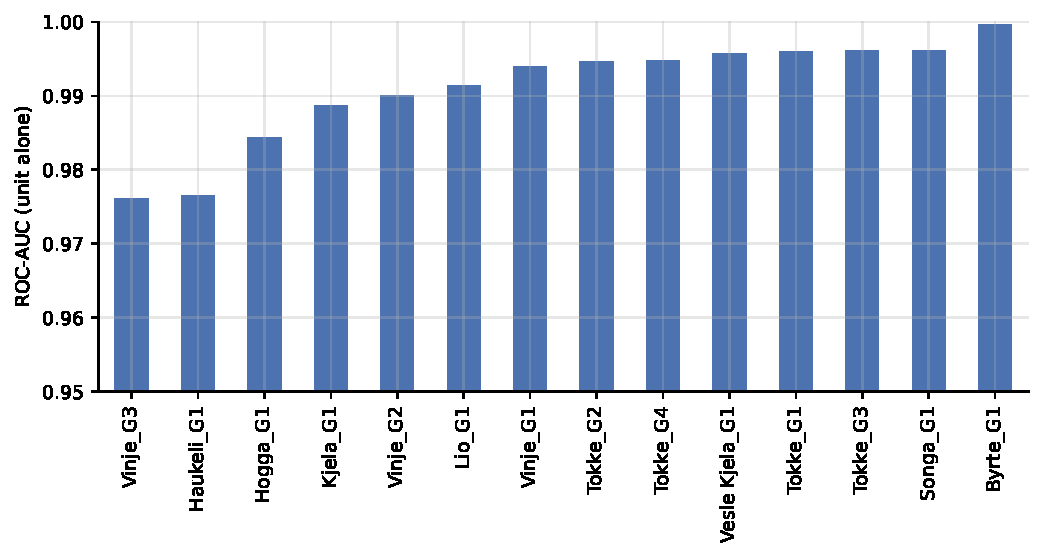
\includegraphics[width=\linewidth]{figures/fig_7_4.pdf}
  \caption{AUC per unit, mean over the four validation years}
  \label{fig:7.4}
\end{figure}

\begin{disposition}
\begin{itemize}
\tightlist
\item
  \emph{Per hour of the horizon (Figure~\ref{fig:7.5}).} The first hours of each case are the hardest (0.989 at hour 0, rising over the first \textasciitilde10 hours), and the last day is the easiest. Explanations: at the start, SHOP knows which units were already running, but we don't (there is no initial on/off state in the data). At the end, decisions are dominated by the +7 d water value, which we know exactly. The curve also dips slightly once a day; see the next point.
\end{itemize}
\end{disposition}

% Final text:


\begin{figure}[H]
  \centering
  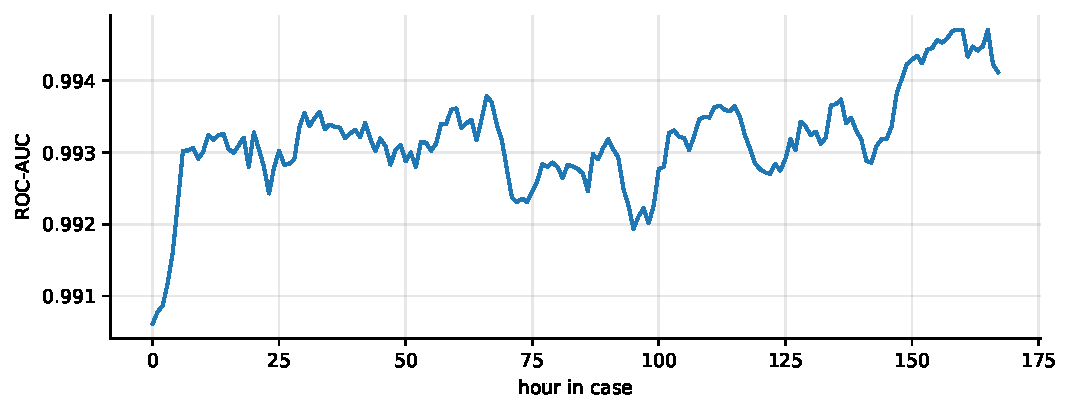
\includegraphics[width=\linewidth]{figures/fig_7_5.pdf}
  \caption{AUC per hour of the horizon (final model, folds A–D)}
  \label{fig:7.5}
\end{figure}

\begin{disposition}
\begin{itemize}
\tightlist
\item
  \emph{The daily dips are at night, not at the switching hours (Table~\ref{tab:7.1}).} Our first guess was that the dips are the hours where units start or stop, since those are the hardest hours to predict. We checked this, and it is wrong:

  \begin{itemize}
  \tightlist
  \item
    The dips are at 23:00--03:00 UTC (midnight to about 04:00 Norwegian time), with AUC 0.991 against 0.992 in the daytime. The difference is small, but it repeats every day.
  \item
    Starts and stops follow the two daily price peaks: units start before the morning peak (04:00--06:00 UTC) and the afternoon peak (15:00--16:00), and stop after them (08:00--11:00 and 18:00--23:00). The AUC in the busiest start hours is normal, and the per-hour AUC is almost unrelated to how many switches happen in that hour (correlation 0.07).
  \item
    What \emph{is} different at night: the simple rule ``price \textgreater{} water value'' fits the decisions slightly worse (81\% vs 83\%), and the model is unsure (probability between 0.2 and 0.8) slightly more often (7.5\% vs 6.6\% of unit-hours).
  \item
    Possible explanation: night prices are low and flat, so for many units the decision is not clearly decided by the price but by other things, for example whether keeping a unit running through the night is cheaper than stopping and restarting it in the morning (start costs), or what the units further up or down the river do. Those are the parts the model captures least well. We have not proven this explanation.
  \end{itemize}
\end{itemize}
\end{disposition}

% Final text:


\begin{table}[H]
  \centering\small
  \caption{Per hour of day (hours 24–167, so the hard first hours do not distort it): AUC, switches, rule fit, model certainty}
  \label{tab:7.1}
  \adjustbox{max width=\linewidth}{\begin{tabular}{p{1.8cm}p{1.2cm}p{1.9cm}p{1.9cm}p{2.6cm}p{2.6cm}}
\toprule
\textbf{Hour of day (UTC)} & \textbf{AUC} & \textbf{Starts (\% of unit-hours)} & \textbf{Stops (\% of unit-hours)} & \textbf{'Price > water value' matches (\%)} & \textbf{Model unsure, 0.2 < p < 0.8 (\%)} \\
\midrule
0 & 0.9908 & 0.0 & 0.9 & 81.4 & 7.5 \\
1 & 0.9908 & 0.1 & 0.6 & 81.2 & 7.6 \\
2 & 0.9908 & 0.2 & 0.3 & 81.1 & 7.6 \\
3 & 0.9912 & 0.9 & 0.1 & 81.5 & 7.4 \\
4 & 0.9915 & 2.3 & 0.1 & 82 & 7.3 \\
5 & 0.9917 & 3.1 & 0.0 & 82.3 & 7 \\
6 & 0.9918 & 2.9 & 0.1 & 82.5 & 6.7 \\
7 & 0.9917 & 1.3 & 0.5 & 82.6 & 6.7 \\
8 & 0.9919 & 0.6 & 1.0 & 82.8 & 6.7 \\
9 & 0.992 & 0.2 & 1.4 & 82.9 & 6.5 \\
10 & 0.992 & 0.1 & 1.2 & 82.8 & 6.6 \\
11 & 0.9921 & 0.0 & 1.0 & 82.8 & 6.6 \\
12 & 0.9921 & 0.1 & 0.5 & 82.8 & 6.7 \\
13 & 0.992 & 0.4 & 0.3 & 82.8 & 6.7 \\
14 & 0.9921 & 0.9 & 0.1 & 82.9 & 6.6 \\
15 & 0.9922 & 1.8 & 0.1 & 83 & 6.6 \\
16 & 0.9921 & 1.6 & 0.2 & 82.8 & 6.7 \\
17 & 0.992 & 0.7 & 0.4 & 82.8 & 6.7 \\
18 & 0.9922 & 0.2 & 1.2 & 82.8 & 6.7 \\
19 & 0.9922 & 0.1 & 1.6 & 82.9 & 6.9 \\
20 & 0.992 & 0.0 & 1.5 & 82.8 & 6.9 \\
21 & 0.9918 & 0.0 & 1.9 & 82.7 & 7 \\
22 & 0.9914 & 0.2 & 1.8 & 82.2 & 7.1 \\
23 & 0.9911 & 0.2 & 1.3 & 82 & 7.2 \\
\bottomrule
\end{tabular}
}
\end{table}

\begin{disposition}
\begin{itemize}
\tightlist
\item
  \emph{Slow optimiser runs (Table~\ref{tab:7.2}).} The data includes how long SHOP took to solve each case (\texttt{total\_calculation\_time}; used only for this analysis, never as a feature). On cases where SHOP took ≥ 900 seconds, our AUC is clearly lower than on fast cases in every year (for example 0.932 vs 0.994 in 2022).

  \begin{itemize}
  \tightlist
  \item
    \emph{Why ``possibly a time limit''.} The labels were made by SINTEF, not by us: they ran SHOP once per case. About half of the slow runs (85 of 174) end at almost the same time, 950--1100 seconds (Section~\ref{sec:2.2}), which looks like SINTEF stopped SHOP at a fixed limit and kept the best schedule found so far. Such a schedule can be slightly worse than the optimal one. The dataset does not say whether there was a limit, so this is our interpretation.
  \item
    \emph{Why we call it ``noise in the validation labels''.} A label is the correct answer we are scored against: SHOP's on/off decision for one unit in one hour. If a slow case was cut off early, some of its labels are not what an optimal SHOP would have chosen. Our model learns the optimal behaviour from the many normal cases, so on a cut-off case its predictions disagree with the labels and the score drops, even though the model is not the problem.
  \item
    \emph{Why down-weighting did not help (exp 032).} Giving the slow cases less weight in training only changes what the model learns. It cannot change the labels the model is scored against, and the model already learns mostly from the normal cases (slow cases are only about 6\% of the training cases). So there was nothing to gain.
  \item
    \emph{Alternative explanation.} The slow cases may simply be hard: several schedules are almost equally profitable, which is exactly why SHOP needed so long to choose. Then the labels are not ``wrong'' but close to arbitrary. Both explanations lead to the same conclusion: this part of the error is a limit of the data, not something a better model can remove.
  \end{itemize}
\end{itemize}
\end{disposition}

% Final text:


\begin{table}[H]
  \centering\small
  \caption{AUC on cases from fast and slow optimiser runs}
  \label{tab:7.2}
  \adjustbox{max width=\linewidth}{\begin{tabular}{lllll}
\toprule
\textbf{year} & \textbf{n fast (< 300 s)} & \textbf{n slow (≥ 900 s)} & \textbf{AUC fast (< 300 s)} & \textbf{AUC slow (≥ 900 s)} \\
\midrule
2019 & 322 & 32 & 0.9948 & 0.9896 \\
2020 & 345 & 15 & 0.9895 & 0.976 \\
2021 & 351 & 7 & 0.9953 & 0.9898 \\
2022 & 344 & 17 & 0.9953 & 0.9341 \\
\bottomrule
\end{tabular}
}
\end{table}

\subsection{One example week}\label{sec:7.4}

\begin{disposition}
Labels, model predictions and the LP's ``unit on'' for four units in a busy 2021 week (1 April; chosen automatically as a week with many on/off switches). What to point out:
\end{disposition}

% Final text:


\begin{figure}[H]
  \centering
  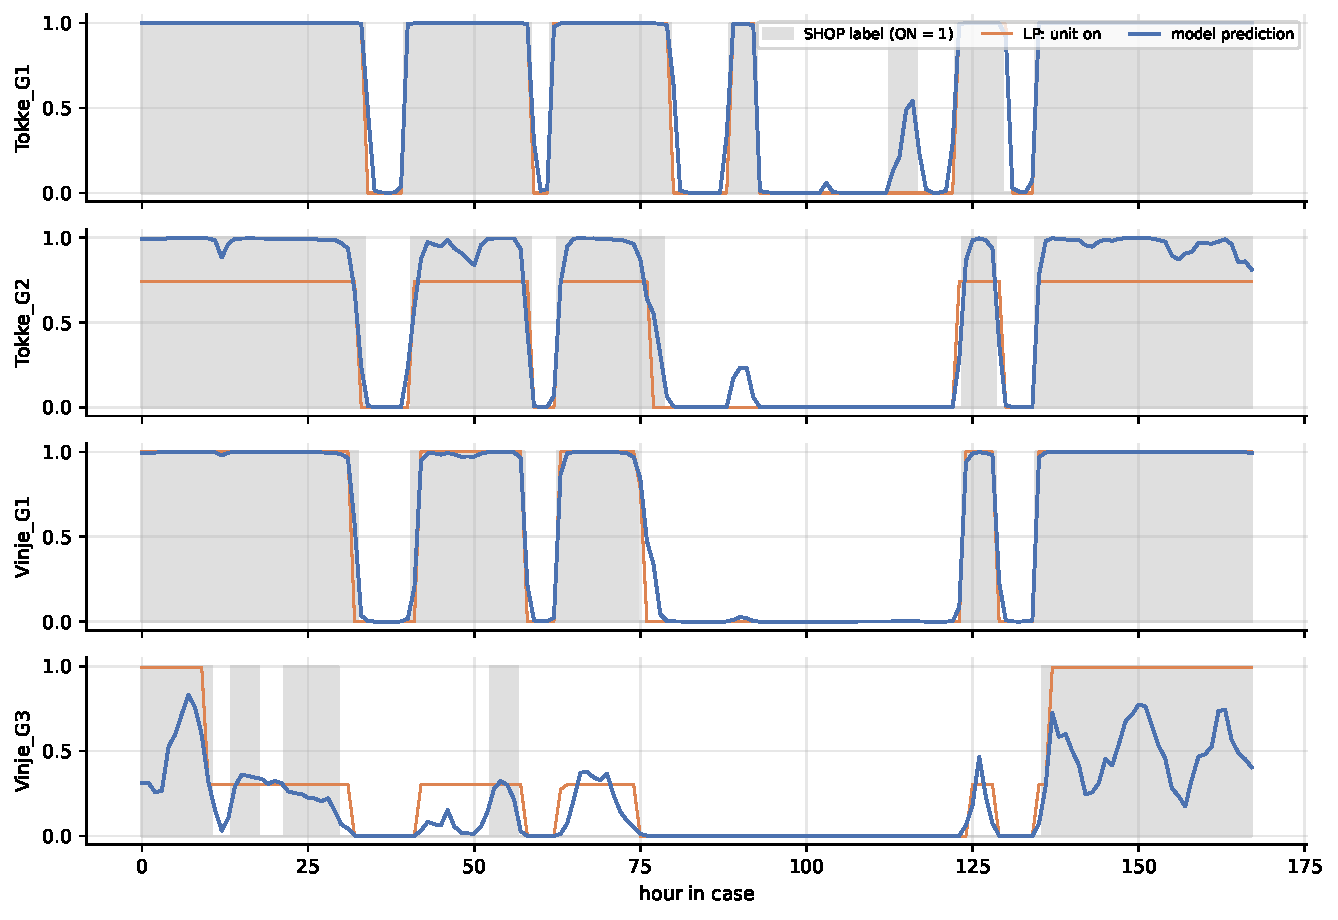
\includegraphics[width=\linewidth]{figures/fig_7_6.pdf}
  \caption{One example week (case starting 2021-04-01): labels, model predictions and the LP's ``unit on'' for four units}
  \label{fig:7.6}
\end{figure}

\begin{disposition}
\begin{itemize}
\tightlist
\item
  \emph{The LP gets the big blocks right.} For Tokke G1 and Vinje G1, the LP's on/off pattern already matches most of SHOP's blocks, and the model follows it.
\item
  \emph{The model sharpens the LP where the LP is fractional.} For Tokke G2 the LP says ``0.75 of a unit'' for whole blocks; the model turns this into close to 1 when SHOP runs the unit and close to 0 when it does not.
\item
  \emph{Uncertainty shows up where it should.} The dips in the model's prediction (e.g.~Vinje G1 around hours 10 and 50) are hours where the decision is close; ranking them in the middle costs little AUC.
\item
  \emph{The weakest unit, Vinje G3, is visibly hard.} SHOP runs it in short blocks in the first 60 hours that neither the LP nor the model predicts, and at the end of the week the LP says ON while the model stays low. This illustrates the near-tie between identical units discussed in 7.3: the model has learned that the LP over-commits the third Vinje unit, so it does not trust it.
\end{itemize}
\end{disposition}

% Final text:

